\documentclass[10pt,twocolumn,a4paper]{article}

\usepackage[utf8]{inputenc}
\usepackage[T1]{fontenc}
\usepackage[italian]{babel}
\usepackage{times}
\usepackage{graphicx}
\usepackage{amsmath}
\usepackage{amssymb}
\usepackage{geometry}
\usepackage{url}
\usepackage{booktabs}
\usepackage{tikz}
\usetikzlibrary{arrows.meta,positioning,shapes.geometric,fit,backgrounds}

\geometry{
	a4paper,
	left=1.6cm,
	right=1.6cm,
	top=1.8cm,
	bottom=2.0cm,
	columnsep=0.7cm
}

\setlength{\parindent}{0.35cm}
\setlength{\parskip}{0pt}

\title{\textbf{PADEL-ANALYZER: A Multi-Head Spatiotemporal Deep Learning
Framework for Independent Team Performance Analytics in Padel}}

\author{
	Dario Ojog\\
	Bachelor's Degree Programme in Applied Computer Science and Artificial Intelligence (ACSAI)\\
	Course: AI-LAB -- Computer Vision, Signal Processing, and Natural Language Processing\\
	Department of Computer Science, Sapienza University of Rome\\
	Matricola: 2135591\\
	\texttt{ojog.2135591@studenti.uniroma1.it}
}

\date{}

\begin{document}

	\maketitle

	\begin{abstract}
		\textbf{PADEL-ANALYZER} è un sistema di \emph{match analytics}
		che, a partire da video reali di partite di padel ripresi da telecamera
		fissa di fondo, ricostruisce la dinamica tattica delle due coppie e ne
		quantifica il comportamento nel tempo. La pipeline rileva i quattro
		giocatori con un detector YOLO, ne proietta il punto-piede su un modello
		metrico del campo ($10\times20$~m) tramite un'omografia, e scarta
		automaticamente replay e cambi di inquadratura mediante un filtro di
		validità geometrico. Le posizioni proiettate vengono raggruppate in
		finestre temporali di dieci frame e classificate da una rete ricorrente
		GRU \emph{multi-head}: un blocco ricorrente condiviso alimenta due teste
		lineari indipendenti, una per squadra, ciascuna delle quali predice uno
		stato posizionale a tre classi (fondo campo, sotto rete, coppia
		disallineata). Il contributo principale è duplice: (i) l'architettura a
		doppia testa modella la \emph{coesistenza} degli stati delle due squadre,
		impossibile con un classificatore a etichetta singola; (ii) ogni stato è
		mappato in una sola delle tre situazioni tattiche (Attacco, Difesa,
		Disallineamento), producendo per ciascuna squadra un report la cui somma
		è esattamente il 100\% del tempo di gioco. Le etichette sono generate in
		modo self-supervised da un'euristica geometrica e la GRU agisce da
		regolarizzatore temporale, riducendo le oscillazioni spurie
		dell'etichetta istantanea. Il sistema produce due report indipendenti con
		la ripartizione percentuale del tempo e una valutazione qualitativa
		automatica delle prestazioni di ciascuna coppia.
	\end{abstract}

	\section{Introduction}

	Lo \emph{sports analytics} è passato in un decennio da una pratica di nicchia
	a uno strumento centrale nella preparazione atletica e tattica, trainato
	dalla disponibilità di video ad alta risoluzione e da modelli di visione
	artificiale sempre più affidabili. Nel padel, sport a crescita rapidissima,
	l'analisi tattica è ancora prevalentemente manuale: un tecnico osserva la
	partita e annota posizioni e transizioni. L'obiettivo di questo progetto è
	automatizzare tale analisi a partire dall'unica fonte realmente disponibile
	per la maggior parte delle partite, ovvero un video di \emph{broadcast}
	ripreso da una telecamera fissa dietro il fondo campo.

	Il problema presenta difficoltà specifiche. In primo luogo, la telecamera
	inquadra il campo in prospettiva: le coordinate immagine non sono
	confrontabili tra loro e vanno riportate a una vista metrica dall'alto. In
	secondo luogo, il flusso di broadcast contiene replay, primi piani e
	grafiche che devono essere riconosciuti e scartati. In terzo luogo, e in
	modo cruciale, la dinamica del padel è \emph{intrinsecamente a due soggetti}:
	le due coppie possono trovarsi contemporaneamente in stati tattici diversi
	(una attacca sotto rete mentre l'altra difende a fondo campo, oppure una
	perde la disposizione mentre l'altra è ordinata). Un classificatore a
	etichetta singola che descriva ``la situazione di gioco'' è quindi
	strutturalmente inadeguato, perché è costretto a collassare due stati
	indipendenti in una sola categoria.

	Le limitazioni degli approcci esistenti che affrontiamo sono dunque: (a) la
	tendenza a usare classificatori mono-testa che non modellano la coesistenza
	degli stati delle due squadre; (b) la fragilità delle analisi rispetto a
	inquadrature non di gioco (replay, primi piani); (c) il costo
	dell'annotazione manuale fotogramma per fotogramma.

	Il contributo di questo progetto è: (1) un'architettura ricorrente \emph{multi-head} con
	blocco GRU condiviso e due teste indipendenti, che predice lo stato delle due
	squadre separatamente e ne modella la coesistenza; (2) una mappatura diretta
	stato~$\rightarrow$~situazione tattica che assegna a ogni squadra, a ogni
	istante, una sola fra tre situazioni (Attacco, Difesa, Disallineamento),
	garantendo report la cui somma è esattamente il 100\%; (3) una strategia di
	etichettatura geometrica self-supervised che rende il sistema addestrabile
	senza annotazioni manuali, con la GRU nel ruolo di regolarizzatore temporale
	delle etichette istantanee rumorose; (4) un filtro di validità basato
	sull'omografia che scarta replay e folla senza modelli aggiuntivi.

	\section{Related Work}
	\label{sec:related}

	\textbf{Rilevamento e tracciamento di giocatori.} Il rilevamento di persone
	in ambito sportivo si basa oggi su detector one-stage della famiglia
	YOLO, che offrono un buon compromesso
	tra accuratezza e velocità in tempo reale. Il tracciamento multi-oggetto è
	spesso aggiunto per mantenere l'identità dei giocatori; nel nostro caso
	l'identità persistente del singolo giocatore non è necessaria: l'assegnazione
	alla squadra deriva deterministicamente dalla metà campo occupata, poiché nel
	padel le coppie non attraversano mai la rete durante il punto.

	\textbf{Omografia e vista dall'alto.} La proiezione delle posizioni su un
	piano metrico tramite omografia è una tecnica consolidata nell'analisi di
	sport di campo, dove i giocatori vengono mappati
	su un modello 2D per calcolare distanze, coperture e formazioni. Applichiamo
	la stessa idea al campo di padel, sfruttando i quattro angoli come
	corrispondenze note.

	\textbf{Analisi temporale e multi-task learning.} Le reti ricorrenti, in
	particolare le GRU, sono efficaci nel modellare sequenze
	temporali brevi come i segnali di posizione. Il \emph{multi-task
	learning} tramite condivisione di parametri è un
	paradigma standard per apprendere obiettivi correlati con un unico backbone;
	lo adottiamo per predire in parallelo, ma indipendentemente, lo stato delle
	due squadre.

	\textbf{Differenza rispetto alla letteratura.} A differenza dei sistemi che
	classificano un'unica ``azione di gioco'' per frame, PADEL-ANALYZER modella
	esplicitamente la coesistenza degli stati con due teste separate e ne deriva
	due report percentuali indipendenti e coerenti (somma $=100\%$). Inoltre
	l'etichettatura self-supervised geometrica evita la costosa annotazione
	manuale dei fotogrammi.

	\section{Methodology}
	\label{sec:method}

	La Fig.~\ref{fig:architecture} riassume l'intera pipeline, dall'input video
	ai due report tattici.

	\begin{figure*}[t]
		\centering
		\begin{tikzpicture}[
			font=\footnotesize,
			node distance=0.55cm and 0.6cm,
			box/.style={draw, rounded corners, align=center, minimum height=0.95cm,
				minimum width=1.9cm, fill=blue!6, thick},
			data/.style={draw, align=center, minimum height=0.95cm,
				minimum width=1.7cm, fill=gray!8},
			head/.style={draw, rounded corners, align=center, minimum height=0.85cm,
				minimum width=1.6cm, fill=green!8, thick},
			arr/.style={-{Latex[length=2mm]}, thick}
			]
			\node[data] (video) {Video\\$1280{\times}720$\\30 fps};
			\node[box, right=of video] (yolo) {YOLO\\person\\detection};
			\node[box, right=of yolo] (homo) {Omografia\\punto-piede\\$\rightarrow$ BEV};
			\node[box, right=of homo] (filt) {Filtro\\validità\\(4 in campo, 2v2)};
			\node[data, right=of filt] (win) {Finestre\\$10{\times}8$};

			\node[box, below=1.15cm of win, fill=orange!10] (gru) {GRU condivisa\\(hidden 64)};
			\node[head, left=1.5cm of gru, yshift=0.55cm] (ha) {Testa A\\3 classi};
			\node[head, left=1.5cm of gru, yshift=-0.55cm] (hb) {Testa B\\3 classi};
			\node[box, left=1.5cm of ha, fill=green!8, yshift=-0.55cm, minimum height=1.5cm] (logic)
			{Mappa stato\\$\rightarrow$\\situazione};
			\node[data, left=of logic, minimum height=1.5cm] (rep) {Report A\\Report B\\(\% tempo)};

			\draw[arr] (video) -- (yolo);
			\draw[arr] (yolo) -- (homo);
			\draw[arr] (homo) -- (filt);
			\draw[arr] (filt) -- (win);
			\draw[arr] (win) -- (gru);
			\draw[arr] (gru.west) -- (ha.east);
			\draw[arr] (gru.west) -- (hb.east);
			\draw[arr] (ha) -- (logic);
			\draw[arr] (hb) -- (logic);
			\draw[arr] (logic) -- (rep);

			\node[above=0.05cm of yolo, font=\scriptsize\itshape] {estrazione};
			\node[above=0.05cm of gru, font=\scriptsize\itshape] {classificazione temporale};
		\end{tikzpicture}
		\caption{Architettura e pipeline di PADEL-ANALYZER. Il video viene
			processato frame per frame: YOLO rileva le persone, l'omografia
			proietta i punti-piede sul campo metrico (Bird's-Eye View), un filtro
			di validità scarta i frame non di gioco. Le posizioni valide sono
			raggruppate in finestre temporali di 10 frame ($8$ feature/frame) e
			classificate da una GRU condivisa con due teste indipendenti (una per
			squadra). Ogni stato predetto viene mappato nella corrispondente
			situazione tattica, generando i due report percentuali.}
		\label{fig:architecture}
	\end{figure*}

	\subsection{Rilevamento e proiezione}

	Per ogni frame, un detector YOLOv8 ristretto alla
	classe \emph{person} restituisce un insieme di bounding box. Da ciascun box
	$[x_1,y_1,x_2,y_2]$ si estrae il \emph{punto-piede}
	$p_{\text{img}}=\big(\tfrac{x_1+x_2}{2},\,y_2\big)$, che approssima il punto
	di contatto del giocatore col suolo ed è più stabile del centroide sotto
	prospettiva.

	\subsection{Omografia}

	La telecamera è fissa, quindi il piano del campo e il piano immagine sono
	legati da un'omografia $\mathbf{H}\in\mathbb{R}^{3\times3}$ stimata una sola
	volta da quattro corrispondenze angolo-campo. Un punto immagine
	$p_{\text{img}}=(u,v)$ si mappa in coordinate metriche $(X,Y)$ tramite
	\begin{equation}
		\tilde{p}_{\text{court}} = \mathbf{H}\,[u,\,v,\,1]^\top,\qquad
		(X,Y)=\Big(\tfrac{\tilde{p}_1}{\tilde{p}_3},\,\tfrac{\tilde{p}_2}{\tilde{p}_3}\Big),
	\end{equation}
	con il campo modellato come rettangolo $[0,10]\times[0,20]$~m e la rete a
	$Y=10$. La calibrazione è ottenuta cliccando i quattro angoli su un
	fotogramma di riferimento; per partite riprese da telecamere diverse la
	calibrazione va ripetuta per ciascun video.

	\subsection{Filtro di validità (scarto dei replay)}

	Un frame è considerato \emph{valido} solo se, dopo la proiezione, restano
	esattamente quattro persone entro i confini logici del campo (con un margine
	di tolleranza di $1.5$~m) e se queste si ripartiscono \emph{due per metà}
	rispetto alla rete. Questo criterio, di natura puramente geometrica, scarta
	simultaneamente il pubblico e l'arbitro (le cui proiezioni cadono fuori
	campo) e i replay o i cambi di inquadratura (in cui il numero o la
	distribuzione dei rilevamenti non rispetta il vincolo $2$ vs $2$). Quando in
	una metà campo vengono rilevate più di due persone, si mantengono le due con
	bounding box di area maggiore (i giocatori, vicini alla telecamera, appaiono
	più grandi degli estranei sullo sfondo).

	\subsection{Etichettatura geometrica self-supervised}

	In assenza di annotazioni manuali, le etichette sono derivate dalla geometria.
	Siano $d_1,d_2$ le distanze dei due giocatori dalla propria rete e
	$\bar{d}=(d_1+d_2)/2$ la profondità media della coppia. Con soglia di
	compattezza $\delta=4$~m e soglia rete/fondo $\tau=5$~m, lo stato $s$ è
	\begin{equation}
		s=\begin{cases}
			2\ (\text{disallineata}) & |d_1-d_2|>\delta,\\
			1\ (\text{rete}) & |d_1-d_2|\le\delta \wedge \bar{d}<\tau,\\
			0\ (\text{fondo}) & |d_1-d_2|\le\delta \wedge \bar{d}\ge\tau.
		\end{cases}
	\end{equation}
	La definizione dello stato \emph{disallineata} in termini di \emph{differenza}
	di profondità fra i due giocatori (anziché di attraversamento di una linea
	fissa) è più aderente alla tattica del padel: una coppia è disorganizzata
	quando un giocatore è marcatamente avanzato rispetto al compagno, non quando
	entrambi sono semplicemente vicini a una soglia. Le etichette istantanee sono
	comunque rumorose vicino a $\delta$ e $\tau$; la rete ricorrente apprende a
	regolarizzarle nel tempo (Sez.~\ref{sec:discussion}). L'effetto di questa
	regolarizzazione è quantificato in Sez.~\ref{sec:setup}, confrontando la GRU
	con la baseline geometrica istantanea.

	\subsection{Finestre temporali e feature}

	I frame validi consecutivi vengono raggruppati in finestre mobili di
	$T=10$ frame; un frame scartato interrompe la continuità. Ogni frame è
	descritto da $8$ feature: le coordinate normalizzate dei quattro giocatori,
	ordinati per metà campo e, all'interno di ciascuna metà, da sinistra a
	destra. L'ordinamento canonico rende la rappresentazione invariante rispetto
	all'ordine di rilevamento.

	\subsection{Rete multi-head e funzione di perdita}

	La sequenza $\mathbf{x}\in\mathbb{R}^{T\times8}$ è processata da una GRU
	condivisa; lo stato dell'ultimo istante
	$\mathbf{h}_T\in\mathbb{R}^{64}$ alimenta due teste lineari indipendenti
	$\mathbf{W}_A,\mathbf{W}_B$ che producono i logit a tre classi
	$\hat{\mathbf{y}}_A,\hat{\mathbf{y}}_B$. L'addestramento è multi-task con
	perdita somma delle due cross-entropy:
	\begin{equation}
		\mathcal{L} = \mathcal{L}_{\text{CE}}(\hat{\mathbf{y}}_A,y_A)
		+ \mathcal{L}_{\text{CE}}(\hat{\mathbf{y}}_B,y_B).
	\end{equation}
	Per contrastare lo sbilanciamento delle classi la cross-entropy è pesata con
	pesi pari alla radice dell'inverso della frequenza, stimati sul solo insieme
	di training: rispetto all'inverso puro, questa scelta attenua la spinta sulle
	classi molto rare (come lo stato \emph{disallineata} della squadra lontana),
	evitando che vengano sistematicamente sovra-predette.

	\subsection{Dallo stato alla situazione tattica}
	\label{sec:logic}

	Ogni stato posizionale predetto è mappato in modo diretto e biunivoco su una
	delle tre situazioni tattiche, che partizionano gli stati e garantiscono che
	la somma dei report di ciascuna squadra sia esattamente il 100\%:
	\begin{equation}
		\sigma(s)=\begin{cases}
			\text{Attacco} & s=1\ (\text{rete}),\\
			\text{Difesa} & s=0\ (\text{fondo}),\\
			\text{Disallineamento} & s=2\ (\text{disallineata}).
		\end{cases}
	\end{equation}
	A partire dalle percentuali il sistema assegna una valutazione qualitativa
	automatica secondo soglie predefinite sul volume d'attacco (${>}40\%$
	DOMINANTE, $25$--$40\%$ OFFENSIVO, ${<}25\%$ PASSIVO) e sul disallineamento
	della coppia (${<}15\%$ COMPATTA, $15$--$30\%$ MOBILE, ${>}30\%$ SLEGATA).

	\subsection{Rilevamento della pallina (modulo complementare)}

	Oltre alla pipeline tattica, un detector dedicato localizza la pallina e ne
	visualizza la traiettoria a video nella demo. L'oggetto è difficile (pochi
	pixel, alta velocità, sfocatura da movimento) e un rilevatore generico è
	inadeguato; abbiamo perciò effettuato il \emph{fine-tuning} di un YOLOv8 su
	alcune centinaia di fotogrammi annotati manualmente per il campo in esame,
	addestrandolo ad alta risoluzione ($1280$~px) per preservare i dettagli fini.
	Un tracker a vicinanza (\emph{nearest-neighbour}) mantiene la continuità della
	traiettoria fra frame. Sul set di demo, mai visto in addestramento, il detector
	individua la pallina in circa il $96\%$ dei frame di gioco, contro una frazione
	molto inferiore di un YOLO generico. Il modulo è specifico per la
	telecamera/campo su cui è annotato.

	\section{Experimental Setup}
	\label{sec:setup}

	\subsection{Dataset}

	Il dataset è costruito da video reali di partite professionistiche di padel
	($1280\times720$, 30 fps) ripresi da telecamera fissa di fondo. Per
	l'addestramento si usano due set distinti, mentre un terzo set è tenuto da
	parte come demo qualitativa e non è mai visto in training. Ogni campione è una
	finestra temporale di 10 frame con due etichette (una per squadra) a tre
	classi. Lo split train/validation/test è \emph{temporale} (70/15/15) ed è
	applicato \emph{all'interno di ciascuna partita}, così ogni set contribuisce a
	tutti e tre gli split e le finestre sovrapposte restano nel medesimo split
	(niente leakage). La Tab.~\ref{tab:dataset} riassume le statistiche ottenute
	dopo il filtro di validità. Un limite noto è che le etichette sono generate da
	un'euristica geometrica anziché da annotazione umana, e che la classe
	\emph{disallineata} è naturalmente meno frequente.

	\begin{table}[h]
		\centering
		\caption{Riepilogo del dataset (aggregato sui due set di training).}
		\label{tab:dataset}
		\begin{tabular}{|l|c|}
			\hline
			\textbf{Proprietà} & \textbf{Valore} \\
			\hline
			Sorgente & Partite professionistiche \\
			Set di training & 2 \\
			Frame totali processati & 124{,}469 \\
			Frame validi (dopo filtro) & 68{,}478 (55.0\%) \\
			Numero di campioni (finestre) & 21{,}720 \\
			Classi (per testa) & 3 \\
			Campioni di training & 15{,}203 \\
			Campioni di validation & 3{,}258 \\
			Campioni di test & 3{,}259 \\
			Formato dell'input & $10\times8$ (temporale) \\
			\hline
		\end{tabular}
	\end{table}

	\subsection{Training and Evaluation Protocol}

	Gli esperimenti sono eseguiti in Python con PyTorch e Ultralytics; la
	detection sfrutta la GPU. La rete è addestrata con Adam, perdita
	cross-entropy pesata sommata sulle due teste. La Tab.~\ref{tab:training}
	riporta la configurazione. Le metriche sono accuratezza e F1 macro per
	ciascuna testa, valutate sul test set; come diagnosi qualitativa si usano le
	matrici di confusione e la stabilità temporale delle predizioni.

	\begin{table}[h]
		\centering
		\caption{Configurazione di training.}
		\label{tab:training}
		\begin{tabular}{|l|c|}
			\hline
			\textbf{Parametro} & \textbf{Valore} \\
			\hline
			Framework & PyTorch \\
			Detector & YOLOv8m (Ultralytics) \\
			Backbone temporale & GRU, hidden 64, 1 layer \\
			Optimizer & Adam \\
			Learning rate & $10^{-3}$ \\
			Batch size & 128 \\
			Epochs & 40 \\
			Loss & $\mathcal{L}_A+\mathcal{L}_B$ (CE pesata) \\
			Metrica principale & Accuracy / F1 macro \\
			\hline
		\end{tabular}
	\end{table}

	\subsection{Results}

	La Tab.~\ref{tab:results} riporta le prestazioni della GRU multi-head sul test
	set, separatamente per le due teste. La testa della Squadra~A (lato vicino) è
	la più bilanciata e leggibile; la testa della Squadra~B (lato lontano) soffre
	della rarità dello stato \emph{disallineata}, che ne abbassa l'F1 macro. Le
	Fig.~\ref{fig:loss} e~\ref{fig:cm} mostrano le curve di apprendimento e le
	matrici di confusione sul test set; queste ultime evidenziano che la classe
	\emph{disallineata} è la più difficile, specie per la Squadra~B.

	\begin{table}[h]
		\centering
		\caption{Prestazioni della GRU multi-head sul test set.}
		\label{tab:results}
		\begin{tabular}{|l|c|c|}
			\hline
			\textbf{Testa} & \textbf{Accuratezza} & \textbf{F1 macro} \\
			\hline
			Squadra A (lato vicino)  & 0.94 & 0.92 \\
			Squadra B (lato lontano) & 0.91 & 0.79 \\
			\hline
		\end{tabular}
	\end{table}

	\begin{figure}[h]
		\centering
		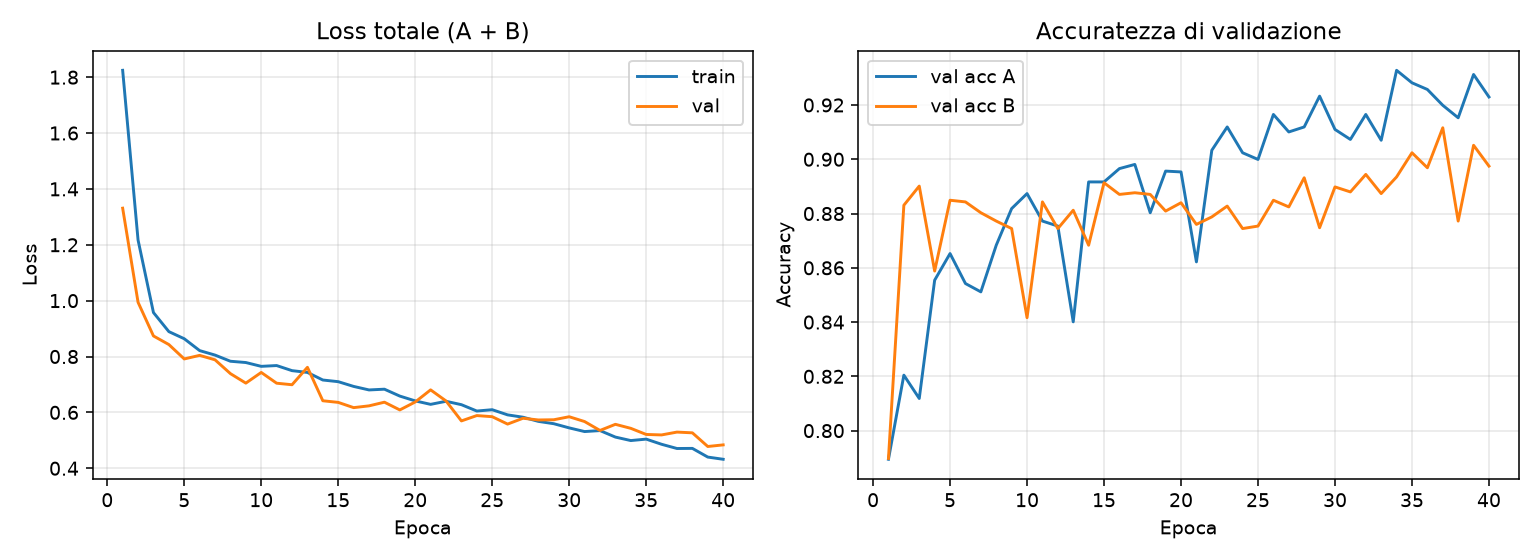
\includegraphics[width=0.98\columnwidth]{loss_plot.png}
		\caption{Curve di apprendimento: loss totale (train/val) e accuratezza di
			validazione delle due teste.}
		\label{fig:loss}
	\end{figure}

	\begin{figure}[h]
		\centering
		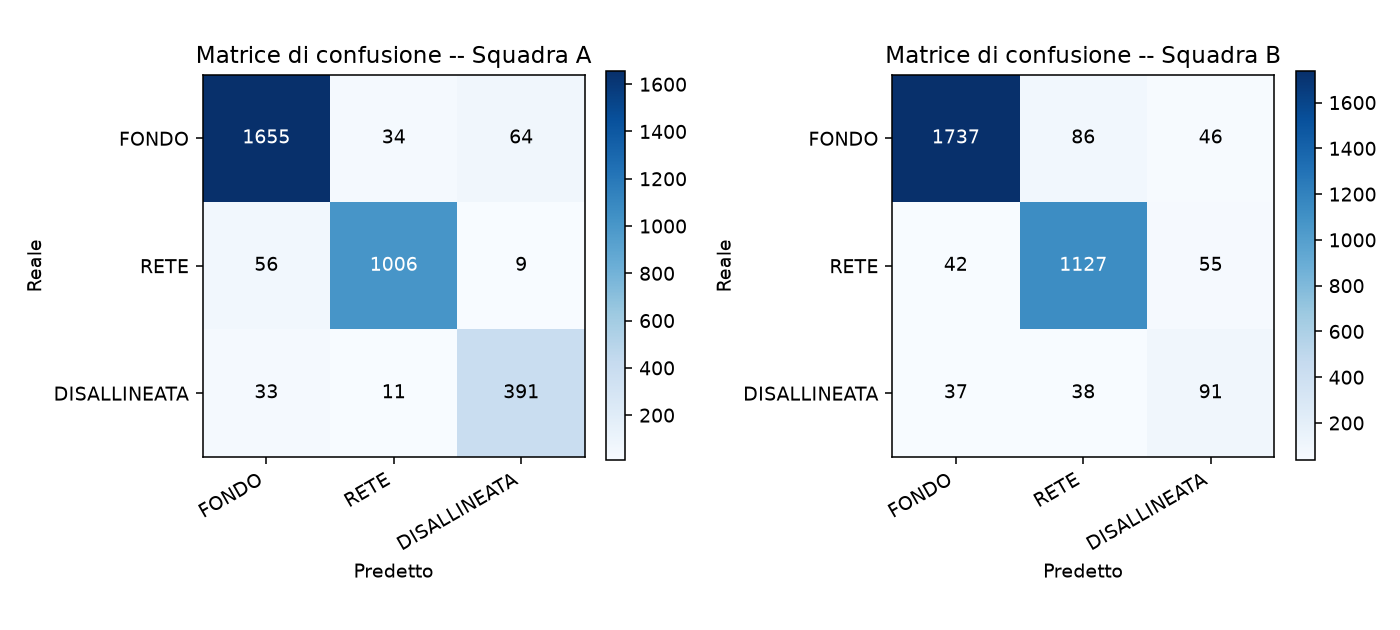
\includegraphics[width=0.98\columnwidth]{confusion_matrix.png}
		\caption{Matrici di confusione sul test set per la testa della Squadra A
			(sinistra) e della Squadra B (destra).}
		\label{fig:cm}
	\end{figure}

	Applicando il modello all'intero materiale analizzato ($64{,}936$ finestre a
	passo unitario per squadra) si ottengono i due report indipendenti. Per la
	Squadra~A la ripartizione è Attacco $33.7\%$, Difesa $53.6\%$, Disallineamento
	$12.7\%$; per la Squadra~B Attacco $36.4\%$, Difesa $56.6\%$, Disallineamento
	$7.0\%$. Ogni report somma esattamente al $100\%$, per costruzione della
	mappatura stato~$\rightarrow$~situazione (Sez.~\ref{sec:logic}).

	\textbf{Confronto con la baseline.} La baseline naturale è la classificazione
	geometrica istantanea, che assegna lo stato frame per frame senza contesto
	temporale. La confrontiamo con la GRU sulla \emph{stabilità temporale},
	contando i cambi di stato fra frame consecutivi: la baseline produce $27.5$
	transizioni/minuto, la GRU $19.4$ (riduzione del $29.6\%$). La rete ricorrente
	rimuove circa un terzo delle oscillazioni spurie prodotte dall'euristica
	frame-per-frame, confermando il ruolo di regolarizzatore temporale e il valore
	aggiunto del contesto rispetto alla classificazione istantanea.

	\subsection{Critical Discussion}
	\label{sec:discussion}

	\textbf{Coesistenza degli stati.} Il risultato metodologico principale è che,
	grazie all'architettura a due teste, il sistema descrive le due squadre in
	modo indipendente e simultaneo: ogni frame contribuisce a una e una sola
	situazione per squadra, e la somma di ciascun report è esattamente il 100\%
	per costruzione. Un classificatore mono-testa avrebbe dovuto scegliere una
	sola etichetta anche quando le due squadre si trovano in stati opposti (una
	attacca, l'altra difende), introducendo un doppio conteggio o una perdita
	d'informazione.

	\textbf{Ruolo della GRU.} Poiché le etichette sono geometriche, la rete non
	apprende una ``verità'' tattica esterna ma una versione temporalmente
	coerente dell'euristica: agisce da filtro che riduce le oscillazioni spurie
	dello stato vicino alle soglie $\delta$ e $\tau$. La riduzione dei cambi di
	stato al minuto (Sez.~\ref{sec:setup}) quantifica questo beneficio, che è il
	valore aggiunto del contesto temporale rispetto alla classificazione
	istantanea. Il rovescio della medaglia emerge sulla Squadra~B, dove la rarità
	della classe \emph{disallineata} e l'uso di pesi di classe inducono un
	compromesso fra recall della classe minoritaria e accuratezza complessiva.

	\textbf{Limiti fisici.} Il limite dominante è visivo: le occlusioni tra i
	corpi dei giocatori, frequenti quando la coppia è vicina o quando i due
	giocatori lontani si sovrappongono alla struttura della rete, producono
	rilevamenti mancati o punti-piede imprecisi. In tali frame il vincolo
	``4 giocatori, 2 vs 2'' fallisce e il frame viene scartato, riducendo la
	copertura. Un secondo limite è la sensibilità dell'omografia alla
	calibrazione: piccoli errori sui quattro angoli si propagano sulle coordinate
	metriche e quindi sulle soglie di stato. Infine, l'etichettatura
	self-supervised eredita i bias dell'euristica e la classe \emph{disallineata}
	resta sotto-rappresentata, come visibile nelle matrici di confusione.
	Sviluppi futuri includono un tracker per stabilizzare le identità, una
	calibrazione automatica basata sul riconoscimento delle linee, la
	validazione delle etichette geometriche contro un insieme annotato più ampio
	e lo sfruttamento del ball tracking per un'analisi più approfondita della partita.

	\section{Conclusion}
	\label{sec:concl}

	Abbiamo presentato PADEL-ANALYZER, una pipeline completa che trasforma i video
	di broadcast di padel in due report tattici indipendenti per le due coppie. Il
	sistema combina detection YOLO, proiezione omografica, filtro di validità
	geometrico ed una GRU multi-head addestrata in regime multi-task su etichette
	geometriche self-supervised. Il contributo centrale è l'aver modellato la
	coesistenza degli stati con due teste indipendenti e l'aver derivato due
	report percentuali coerenti tramite una mappatura diretta stato-situazione. I
	limiti principali riguardano le occlusioni visive e la dipendenza dalla
	calibrazione; le direzioni future puntano a etichette parzialmente
	supervisionate e a una calibrazione automatica.

	\section*{Acknowledgments}

	Il progetto utilizza le librerie open-source PyTorch e Ultralytics YOLO e
	video di partite ufficiali come sorgente dati.

	\begin{figure*}[p]
		\centering
		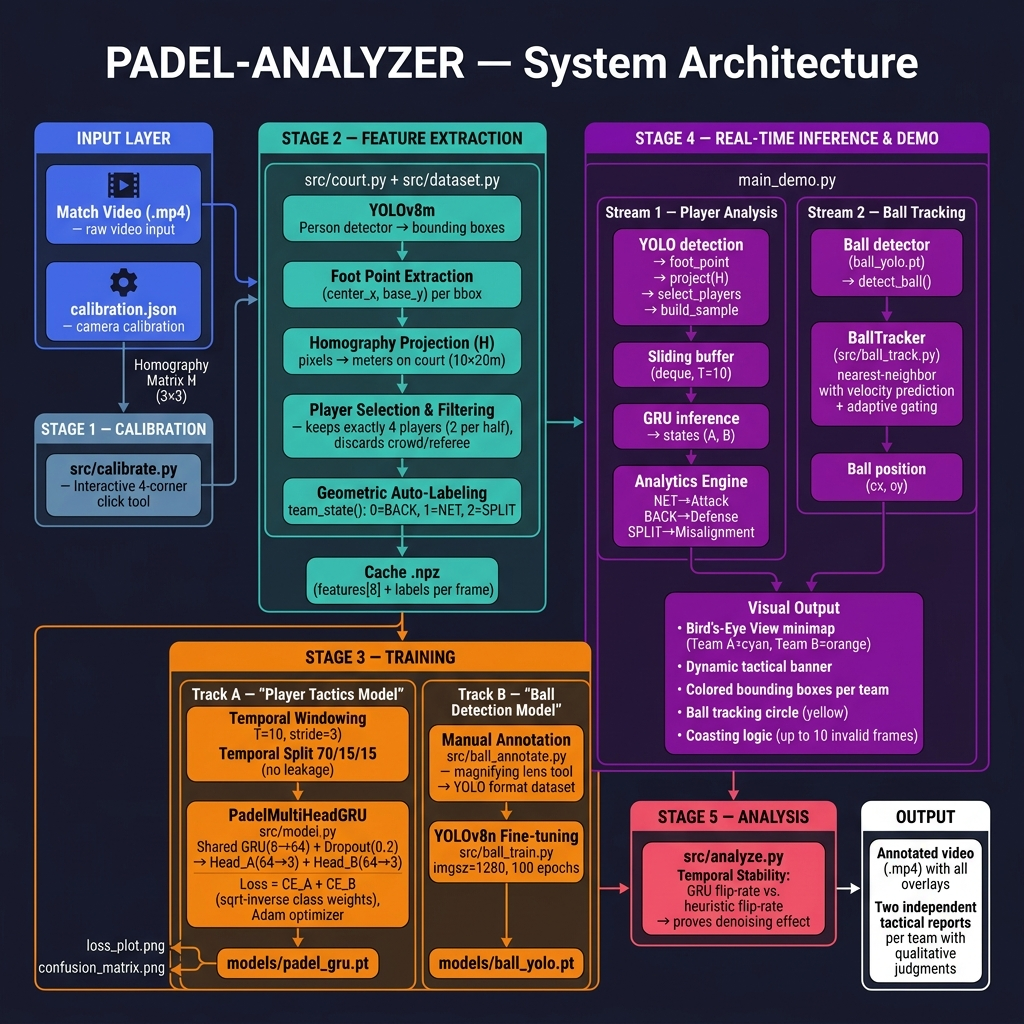
\includegraphics[width=0.92\textwidth]{Architettura.png}
		\caption{Schema completo dell'architettura di sistema: calibrazione,
			estrazione delle feature, training (modello tattico e detector della
			pallina) e pipeline di inferenza/demo.}
		\label{fig:full-architecture}
	\end{figure*}

\end{document}
